% 第15章第3节：秩k逼近（子空间选择与迹极值、截断SVD的构造、最佳误差与最优性、最优解的唯一性）。

\section{秩\texorpdfstring{$k$}{k}逼近}
\label{sec:ls-low-rank-approximation}
\label{sec:ls-low-rank-solve}
\label{sec:ls-full-svd-solve}
\label{sec:matrix-analysis-svd-low-rank}

把共同的重建方向由一条直线扩展为$k$维子空间。与秩一情形一样，先固定子空间求系数，再选择子空间本身；用子空间的标准正交基，保留量写成一个迹，选子空间就成为迹的极值问题。由奇异值分解可以写出这个问题的解，即截断SVD；随后在Frobenius范数与谱范数下证明它的最优性，并讨论最优解何时唯一。

\subsection{子空间选择与迹极值}
\label{sec:ls-low-rank-projection-error}
\label{sec:ls-rank-k-trace}

\paragraph{固定子空间时的最优重建}
秩约束要求全部重建向量共用至多$k$个独立方向。先把这些方向张成的$k$维子空间固定下来，问每一列应当怎样重建。直观上，答案应当是把每一列正交投影到这个子空间上，这与秩一情形相同；下面把这一点写成等式。

以列标准正交的$\bm Y\in\mathbb R^{m\times k}$表示这个子空间，
\[
 \bm Y^\top\bm Y=\bm I_k ;
\]
这里不用字母$\bm V$，以免与右奇异向量矩阵混淆。列都落在$\operatorname{range}(\bm Y)$中的矩阵恰好是
\[
 \bm X=\bm Y\bm C,\qquad \bm C\in\mathbb R^{k\times d},
\]
$\bm C$的第$j$列是$\bm x_j$在这组基下的系数。由第~\ref{chap:inner-product-spaces}章的投影矩阵，$\bm Y\bm Y^\top$是到$\operatorname{range}(\bm Y)$的正交投影。

以$m=3$、$k=2$、$\bm Y=[\bm e_1,\bm e_2]$为例，按元素写出
\[
 \begin{gathered}
 \bm Y\bm Y^\top=\begin{bmatrix}1&0&0\\0&1&0\\0&0&0\end{bmatrix},\\
 \bm Y\bm C=\begin{bmatrix}c_{1,1}&\cdots&c_{1,d}\\c_{2,1}&\cdots&c_{2,d}\\0&\cdots&0\end{bmatrix}.
 \end{gathered}
\]
投影保留每一列的前两个分量、去掉第三个分量；候选矩阵的第三行只能是零，前两行可以任意选取。

\begin{lemma}[固定子空间时的正交误差分解]
\label{lem:ls-low-rank-projection-error}
设$\bm Y\in\mathbb R^{m\times k}$满足$\bm Y^\top\bm Y=\bm I_k$，则对任意$\bm C\in\mathbb R^{k\times d}$，
\begin{equation}
 \begin{aligned}
 \lVert\bm A-\bm Y\bm C\rVert_{\mathrm F}^2
 &=\lVert(\bm I-\bm Y\bm Y^\top)\bm A\rVert_{\mathrm F}^2\\
 &\qquad+\lVert\bm Y^\top\bm A-\bm C\rVert_{\mathrm F}^2,
 \end{aligned}
 \label{eq:ls-low-rank-projection-split}
\end{equation}
并且
\begin{equation}
 \lVert(\bm I-\bm Y\bm Y^\top)\bm A\rVert_{\mathrm F}^2
 =\lVert\bm A\rVert_{\mathrm F}^2-\operatorname{tr}(\bm Y^\top\bm A\bm A^\top\bm Y).
 \label{eq:ls-low-rank-projection-residual}
\end{equation}
因此固定子空间时，最优系数唯一，为$\bm C=\bm Y^\top\bm A$，最优重建是正交投影$\bm Y\bm Y^\top\bm A$。
\end{lemma}
\begin{proof}
把误差矩阵拆成两部分：
\[
 \bm A-\bm Y\bm C=(\bm I-\bm Y\bm Y^\top)\bm A+\bm Y(\bm Y^\top\bm A-\bm C).
\]
逐列看，第$j$列是$\bm r_j=(\bm I-\bm Y\bm Y^\top)\bm a_j$与$\bm Y\bm z_j$之和，其中$\bm z_j$是$\bm Y^\top\bm A-\bm C$的第$j$列。二者正交：
\[
 \bm r_j^\top\bm Y\bm z_j=\bm a_j^\top(\bm I-\bm Y\bm Y^\top)\bm Y\bm z_j
 =\bm a_j^\top(\bm Y-\bm Y\bm Y^\top\bm Y)\bm z_j=0 ,
\]
这里用到$\bm Y^\top\bm Y=\bm I_k$。又由同一关系，
\[
 \lVert\bm Y\bm z_j\rVert_2^2=\bm z_j^\top\bm Y^\top\bm Y\bm z_j=\lVert\bm z_j\rVert_2^2 .
\]
由勾股定理，误差矩阵第$j$列的平方长度是
\[
 \lVert\bm r_j\rVert_2^2+\lVert\bm z_j\rVert_2^2 ;
\]
对$j$求和即得式~\eqref{eq:ls-low-rank-projection-split}。

对第二式，同样把$\bm a_j$分解为$\bm Y\bm Y^\top\bm a_j$与$\bm r_j$两个正交部分，得
\[
 \lVert\bm r_j\rVert_2^2=\lVert\bm a_j\rVert_2^2-\lVert\bm Y^\top\bm a_j\rVert_2^2 .
\]
求和后，
\[
 \sum_j\lVert\bm Y^\top\bm a_j\rVert_2^2=\lVert\bm Y^\top\bm A\rVert_{\mathrm F}^2
 =\operatorname{tr}(\bm Y^\top\bm A\bm A^\top\bm Y).
\]
最后，式~\eqref{eq:ls-low-rank-projection-split}右端第一项与$\bm C$无关，第二项非负，且当且仅当$\bm C=\bm Y^\top\bm A$时为零。
\end{proof}

于是在固定子空间中，误差等于总平方长度减去保留量$\operatorname{tr}(\bm Y^\top\bm A\bm A^\top\bm Y)$；$k=1$、$\bm Y=\bm u$时，这正是第~\ref{sec:matrix-approximation-rank-one-coefficients}节逐列配方得到的公式。示例~\ref{ex:ls-low-rank-three-columns}中“先投影再计损失”的做法，也正是这个最优重建。

共同子空间把$d$个向量各自的最小二乘问题合成了一个矩阵近似问题：子空间共用，系数逐列由投影给出。

在上面$\bm Y=[\bm e_1,\bm e_2]$的例子中，取$\bm A=\operatorname{diag}(3,2,1)$，最优系数与最优重建为
\[
 \begin{gathered}
 \bm Y^\top\bm A=\begin{bmatrix}3&0&0\\0&2&0\end{bmatrix},\\
 \bm Y\bm Y^\top\bm A=\begin{bmatrix}3&0&0\\0&2&0\\0&0&0\end{bmatrix}.
 \end{gathered}
\]
残差只剩右下角的$1$，平方误差为
\[
 \lVert\bm A\rVert_{\mathrm F}^2-\operatorname{tr}(\bm Y^\top\bm A\bm A^\top\bm Y)=14-(9+4)=1 ,
\]
与示例~\ref{ex:ls-low-rank-three-columns}中坐标平面$\operatorname{span}\{\bm e_1,\bm e_2\}$的损失一致。

\paragraph{化为子空间的选择}
引理只处理了列都落在给定子空间中的候选。下面说明，这一化归覆盖全部秩不超过$k$的矩阵，而不只覆盖事先写成投影形式的矩阵。

设$\operatorname{rank}\bm X=s\leq k$。取$\bm X$列空间的一组标准正交基，再在$\mathbb R^m$中补充$k-s$个与之正交的单位向量（$k\leq m$，所以可以补齐），排成$\bm Y$。则$\bm X$的列都落在$\operatorname{range}(\bm Y)$中，
\[
 \bm X=\bm Y\bm C,\qquad \bm C=\bm Y^\top\bm X .
\]
由引理~\ref{lem:ls-low-rank-projection-error}，
\[
 \lVert\bm A-\bm X\rVert_{\mathrm F}^2\geq\lVert\bm A\rVert_{\mathrm F}^2-\operatorname{tr}(\bm Y^\top\bm A\bm A^\top\bm Y).
\]
反过来，每个列标准正交的$\bm Y$都给出秩不超过$k$的候选$\bm Y\bm Y^\top\bm A$，误差恰为右端。两方面合起来，
\begin{equation}
 \begin{aligned}
 &\min_{\operatorname{rank}\bm X\leq k}\lVert\bm A-\bm X\rVert_{\mathrm F}^2\\
 &\qquad=\lVert\bm A\rVert_{\mathrm F}^2-\max_{\bm Y^\top\bm Y=\bm I_k}\operatorname{tr}(\bm Y^\top\bm A\bm A^\top\bm Y),
 \end{aligned}
 \label{eq:ls-low-rank-subspace-reduction}
\end{equation}
只要右端的最大值存在；最大值的存在与取值由下面的定理~\ref{thm:matrix-analysis-trace-minimum}给出。到这里，“同时选择方向与系数”化成了“选择子空间”。

\paragraph{保留量的含义}
再看保留量本身。对$\bm Y=[\bm y_1,\ldots,\bm y_k]$按列展开：
\[
 \begin{aligned}
 \operatorname{tr}(\bm Y^\top\bm A\bm A^\top\bm Y)
 &=\sum_{l=1}^k\bm y_l^\top\bm A\bm A^\top\bm y_l\\
 &=\sum_{l=1}^k\sum_{j=1}^d(\bm y_l^\top\bm a_j)^2 .
 \end{aligned}
\]
迹把$k$个互相垂直方向上的保留量相加，$k=1$时恰好回到上一节的Rayleigh商。

保留量只依赖子空间，不依赖基的选取。记$\bm G=\bm A\bm A^\top$。把$\bm Y$换成$\bm Y\bm O$（$\bm O$为$k$阶正交矩阵）时，由迹的循环性，
\[
 \operatorname{tr}(\bm O^\top\bm Y^\top\bm G\bm Y\bm O)=\operatorname{tr}(\bm Y^\top\bm G\bm Y).
\]

据此，由式~\eqref{eq:ls-low-rank-subspace-reduction}，秩$k$逼近归结为下面的\emph{迹极值问题}：
\[
 \begin{gathered}
 \text{在}\ \bm Y^\top\bm Y=\bm I_k\ \text{下最大化}\ \operatorname{tr}(\bm Y^\top\bm G\bm Y),\\
 \bm G=\bm A\bm A^\top .
 \end{gathered}
\]

\paragraph{两个候选界}
逐列套用Rayleigh--Ritz定理只能得到每一项不超过$\lambda_1(\bm G)$，即
\[
 \operatorname{tr}(\bm Y^\top\bm G\bm Y)\leq k\lambda_1(\bm G).
\]
这个界没有用到各列互相正交的约束，一般取不到：由定理~\ref{thm:matrix-analysis-rayleigh-ritz}的取等条件，总和等于$k\lambda_1(\bm G)$要求每个$\bm y_l$都落在最大特征值的特征空间中；若$\lambda_1(\bm G)$单重，这个特征空间是一条直线，$k\geq2$时容不下$k$个互相正交的单位向量。

另一个方向是只比较由$\bm G$的特征向量组成的子空间。设$\bm G$的特征值为$\lambda_1\geq\cdots\geq\lambda_m$，对应标准正交特征向量$\bm q_1,\ldots,\bm q_m$。取$\bm Y=[\bm q_{i_1},\ldots,\bm q_{i_k}]$（下标互不相同），则$\bm y_l^\top\bm G\bm y_l=\lambda_{i_l}$，保留量为
\[
 \operatorname{tr}(\bm Y^\top\bm G\bm Y)=\lambda_{i_1}+\cdots+\lambda_{i_k}.
\]
保留前$k$个特征方向给出最大的特征值和$\sum_{i\leq k}\lambda_i$。

回到示例~\ref{ex:ls-low-rank-three-columns}，$\bm G=\operatorname{diag}(9,4,1)$。第一个界给出$2\times9=18$，超过总长度平方$14$，显然太松。三个坐标平面给出$13,10,5$，其中前两个特征方向张成的$\operatorname{span}\{\bm e_1,\bm e_2\}$最好，保留$13$、损失$1$。

一般地，由式~\eqref{eq:ls-svd-transpose-relation}，$\bm A\bm A^\top$的前$k$个特征方向可以取为左奇异向量$\bm u_1,\ldots,\bm u_k$，候选子空间就是$\operatorname{span}\{\bm u_1,\ldots,\bm u_k\}$。

\paragraph{倾斜子空间与权重}
任意倾斜的子空间会把权重分散到多个特征方向上，它是否仍不能超过特征值和，需要看清正交约束对权重的限制。仍取$\bm G=\operatorname{diag}(9,4,1)$，考虑倾斜平面
\[
 \bm Y=\begin{bmatrix}1&0\\0&1/\sqrt2\\0&1/\sqrt2\end{bmatrix}.
\]
它在三个特征方向$\bm e_1,\bm e_2,\bm e_3$上的权重$w_i=\lVert\bm Y^\top\bm e_i\rVert_2^2$依次是$\bm Y$各行的平方长度：
\[
 w_1=1,\qquad w_2=\frac12,\qquad w_3=\frac12 .
\]
保留量就是特征值的加权和：
\[
 \operatorname{tr}(\bm Y^\top\bm G\bm Y)=9\cdot1+4\cdot\frac12+1\cdot\frac12=\frac{23}2<13 .
\]
权重各不超过$1$，总和为$k=2$。这个平面把第二个特征方向上的一半权重让给了较小的第三个特征值，因而保留得更少。

下面的定理说明这对任意实对称矩阵、任意$k$维子空间都成立；同时也回答迹能否低于后$k$个特征值之和。

\begin{theorem}[迹极值]
\label{thm:matrix-analysis-trace-minimum}
设$\bm S\in\mathbb R^{m\times m}$实对称，特征值$\lambda_1\geq\cdots\geq\lambda_m$，对应标准正交特征向量$\bm q_1,\ldots,\bm q_m$，$1\leq k\leq m$。对满足$\bm Y^\top\bm Y=\bm I_k$的$\bm Y\in\mathbb R^{m\times k}$，
\begin{equation}
 \sum_{i=m-k+1}^{m}\lambda_i\leq\operatorname{tr}(\bm Y^\top\bm S\bm Y)\leq\sum_{i=1}^{k}\lambda_i,
 \label{eq:matrix-analysis-trace-minimum}
\end{equation}
上界由$\bm Y=[\bm q_1,\ldots,\bm q_k]$取到，下界由$\bm Y=[\bm q_{m-k+1},\ldots,\bm q_m]$取到。若$k<m$且$\lambda_k>\lambda_{k+1}$，则上界取等当且仅当$\operatorname{range}(\bm Y)=\operatorname{span}\{\bm q_1,\ldots,\bm q_k\}$。
\end{theorem}
\begin{proof}
由谱定理，$\bm S=\sum_i\lambda_i\bm q_i\bm q_i^\top$，故
\[
 \operatorname{tr}(\bm Y^\top\bm S\bm Y)
 =\sum_{i=1}^m\lambda_i\operatorname{tr}(\bm Y^\top\bm q_i\bm q_i^\top\bm Y)
 =\sum_{i=1}^m\lambda_iw_i,
\]
其中$w_i=\lVert\bm Y^\top\bm q_i\rVert_2^2$。权重受两条限制。

第一，$\bm P=\bm Y\bm Y^\top$是到$\operatorname{range}(\bm Y)$的正交投影，满足$\bm P=\bm P^\top\bm P$，所以
\[
 w_i=\bm q_i^\top\bm P\bm q_i=\bm q_i^\top\bm P^\top\bm P\bm q_i=\lVert\bm P\bm q_i\rVert_2^2 .
\]
正交投影不增加长度，所以$0\leq w_i\leq\lVert\bm q_i\rVert_2^2=1$。

第二，记$\bm Q=[\bm q_1,\ldots,\bm q_m]$，它是正交矩阵，右乘正交矩阵不改变Frobenius范数，于是
\[
 \sum_{i=1}^mw_i=\lVert\bm Y^\top\bm Q\rVert_{\mathrm F}^2=\lVert\bm Y^\top\rVert_{\mathrm F}^2=\operatorname{tr}(\bm Y^\top\bm Y)=k .
\]
也就是说，总量为$k$的权重分配给各个特征值，每个特征值至多分到$1$。

直观上，要使加权和最大，应把权重全部放在最大的$k$个特征值上。用$\lambda_k$作为分界，可以把这一直观写成恒等式：
\[
 \begin{aligned}
 \sum_{i=1}^m\lambda_iw_i-\sum_{i=1}^k\lambda_i
 &=\sum_{i\leq k}(\lambda_i-\lambda_k)(w_i-1)+\sum_{i>k}(\lambda_i-\lambda_k)w_i\\
 &\qquad+\lambda_k\Bigl(\sum_{i=1}^mw_i-k\Bigr).
 \end{aligned}
\]
展开右端即可核对。最后一项因$\sum_iw_i=k$而为零。$i\leq k$时$\lambda_i-\lambda_k\geq0$、$w_i-1\leq0$；$i>k$时$\lambda_i-\lambda_k\leq0$、$w_i\geq0$。所以右端每一项都不大于零，上界成立。

上界可以取到：$\bm Y=[\bm q_1,\ldots,\bm q_k]$时$w_i$在$i\leq k$时为$1$、其余为$0$，迹等于$\sum_{i\leq k}\lambda_i$。

取等条件也可以从这个恒等式读出。若$\lambda_k>\lambda_{k+1}$，则$i>k$时$\lambda_i-\lambda_k<0$，上界取等迫使$w_i=0$，即$\bm Y^\top\bm q_i=\bm0$。于是$\operatorname{range}(\bm Y)$与$\bm q_{k+1},\ldots,\bm q_m$都正交，含于$\operatorname{span}\{\bm q_1,\ldots,\bm q_k\}$；两者都是$k$维的，所以相等。

反之，若$\operatorname{range}(\bm Y)=\operatorname{span}\{\bm q_1,\ldots,\bm q_k\}$，则$i\leq k$时$\bm P\bm q_i=\bm q_i$、$i>k$时$\bm P\bm q_i=\bm0$，迹等于上界。

下界由上界得到。$-\bm S$的特征值按降序为$-\lambda_m\geq\cdots\geq-\lambda_1$，对应特征向量依次为$\bm q_m,\ldots,\bm q_1$。对$-\bm S$应用上界，得
\[
 -\operatorname{tr}(\bm Y^\top\bm S\bm Y)\leq-\sum_{i=m-k+1}^m\lambda_i ,
\]
等号在$\bm Y=[\bm q_{m-k+1},\ldots,\bm q_m]$时成立。
\end{proof}

在倾斜平面的例子中，恒等式右端的三类项分别是
\[
 (9-4)(1-1)=0,\qquad (4-4)\Bigl(\frac12-1\Bigr)=0,\qquad (1-4)\cdot\frac12=-\frac32 .
\]
合计$-\tfrac32$，正是$\tfrac{23}2-13$：亏损全部来自让给第三个特征值的那一半权重。

\paragraph{回到低秩逼近}
取$\bm S=\bm G=\bm A\bm A^\top$。它的特征值是$\sigma_1^2\geq\cdots\geq\sigma_r^2$，再补上$m-r$个零；$k<r$时前$k$个之和为$\sum_{i\leq k}\sigma_i^2$。于是任意$k$维子空间最多保留
\begin{equation}
 \max_{\bm Y^\top\bm Y=\bm I_k}\operatorname{tr}(\bm Y^\top\bm A\bm A^\top\bm Y)=\sum_{i=1}^k\sigma_i^2 ,
 \label{eq:ls-low-rank-max-retained}
\end{equation}
式~\eqref{eq:ls-low-rank-subspace-reduction}右端的最大值存在，并由$\operatorname{span}\{\bm u_1,\ldots,\bm u_k\}$取到。在示例~\ref{ex:ls-low-rank-three-columns}中，这确认任意倾斜平面的保留量都不超过$13$，坐标平面$\operatorname{span}\{\bm e_1,\bm e_2\}$已是最优的平面。

对一般的对称矩阵$\bm S$，迹极值界照样成立，但只有在当前这种半正定的Gram情形，迹才表示投影保留的长度平方。下一小节把最优子空间上的投影重建写成具体的矩阵。

\subsection{截断SVD的构造}
\label{sec:ls-truncated-svd-construction}

\subsubsection{主要思想}

上一小节确定了最优子空间，还没有写出最优重建本身。设$\bm A$的奇异值分解写成和式~\eqref{eq:matrix-analysis-svd-rank-one-sum}，
\[
 \bm A=\sum_{i=1}^r\sigma_i\bm u_i\bm v_i^\top ,
\]
其中$r=\operatorname{rank}\bm A$，$\sigma_1\geq\cdots\geq\sigma_r>0$。$1\leq k<r$时最优子空间可取为$\operatorname{span}\{\bm u_1,\ldots,\bm u_k\}$，即
\[
 \bm Y=\bm U_k=[\bm u_1,\ldots,\bm u_k].
\]
由引理~\ref{lem:ls-low-rank-projection-error}，最优重建是$\bm U_k\bm U_k^\top\bm A$。要把它化简，只需看$\bm U_k^\top$作用在每个$\bm u_i$上的结果。

以$r=3$、$k=2$为例，由$\bm u_i$标准正交，按元素写出
\[
 \bm U_2^\top\bm u_1=\begin{bmatrix}1\\0\end{bmatrix},\qquad
 \bm U_2^\top\bm u_2=\begin{bmatrix}0\\1\end{bmatrix},\qquad
 \bm U_2^\top\bm u_3=\begin{bmatrix}0\\0\end{bmatrix}.
\]
于是$\bm U_2\bm U_2^\top\bm u_i$在$i=1,2$时还原为$\bm u_i$，在$i=3$时为零。一般地，$\bm U_k^\top\bm u_i$在$i\leq k$时等于$\bm e_i$、在$i>k$时等于$\bm0$，所以
\[
 \begin{aligned}
 \bm U_k\bm U_k^\top\bm A
 &=\sum_{i=1}^r\sigma_i\bm U_k(\bm U_k^\top\bm u_i)\bm v_i^\top\\
 &=\sum_{i=1}^k\sigma_i\bm u_i\bm v_i^\top .
 \end{aligned}
\]
也就是说，把$\bm A$的各列正交投影到前$k$个左奇异方向上，等于只保留SVD和式的前$k$项。

把这个由子空间优化推导出的矩阵记下来。对整数$k\geq0$，称
\begin{equation}
\begin{gathered}
\bm A_k=\sum_{i=1}^{\min(k,r)}\sigma_i\bm u_i\bm v_i^\top
 =\bm U_k\bm\Sigma_k\bm V_k^\top\\
k\geq0
\end{gathered}
\label{eq:matrix-analysis-truncated-svd}
\end{equation}
为$\bm A$的\term{截断SVD}（truncated SVD），其中$k\leq r$时$\bm\Sigma_k=\operatorname{diag}(\sigma_1,\ldots,\sigma_k)$，$\bm V_k=[\bm v_1,\ldots,\bm v_k]$。两种边界情形与第~\ref{sec:matrix-approximation-problem}节的直接回答一致：$k=0$时和式为空，$\bm A_0=\bm0$；$k\geq r$时保留了全部项，$\bm A_k=\bm A$。

$\bm A_k$满足秩约束。$k\leq r$时，
\[
 \bm A_k\bm v_i=\sigma_i\bm u_i\quad(i\leq k),\qquad
 \bm A_k\bm v_i=\bm0\quad(i>k),
\]
所以列空间恰为$\operatorname{span}\{\bm u_1,\ldots,\bm u_k\}$，$\operatorname{rank}\bm A_k=k$。

\subsubsection{算法实现}

截断SVD的输入是$\bm A$已经求出的SVD与秩预算$k$，输出是$\bm A_k$或它的三个因子。计算本身不迭代：取出前$k$组奇异值与奇异向量，相乘即可。下面用以下示例中的矩阵逐步演示；它的一个奇异方向是倾斜的，并且有重奇异值。

\begin{example}[有重奇异值的三阶截断]
\label{ex:matrix-approximation-truncated-three-by-three}
取
\[
 \bm A=\begin{bmatrix}3&2&0\\2&3&0\\0&0&1\end{bmatrix}.
\]
令
\[
 \bm u_1=\frac1{\sqrt2}\begin{bmatrix}1\\1\\0\end{bmatrix},\qquad
 \bm u_2=\frac1{\sqrt2}\begin{bmatrix}1\\-1\\0\end{bmatrix},\qquad
 \bm u_3=\begin{bmatrix}0\\0\\1\end{bmatrix},
\]
它们标准正交，且
\[
 \bm A\bm u_1=5\bm u_1,\qquad\bm A\bm u_2=\bm u_2,\qquad\bm A\bm u_3=\bm u_3 .
\]
$\bm A$对称、特征值非负，所以可取$\bm v_i=\bm u_i$，奇异值为$5,1,1$。下面分别取$k=1$与$k=2$。
\end{example}

\paragraph{变量}
\begin{itemize}
 \item $k$：秩预算；$r$：$\bm A$的秩，即正奇异值的个数。
 \item $\sigma_i,\bm u_i,\bm v_i$：已经求出的奇异值与配对的左右奇异向量。
 \item $\bm U_k\in\mathbb R^{m\times k}$、$\bm\Sigma_k$、$\bm V_k\in\mathbb R^{d\times k}$：截取出的三个因子。
 \item $\bm W=\bm\Sigma_k\bm V_k^\top\in\mathbb R^{k\times d}$：缩放后的右因子，即最优系数矩阵。
 \item $\bm A_k$：截断SVD；$\bm E_k=\bm A-\bm A_k$：重建残差，只在核验时形成。
\end{itemize}

\paragraph{输入与预处理}
先核对$k$是满足$0\leq k\leq\min(m,d)$的整数，并由正奇异值的个数确定$r$。$k=0$时直接输出零矩阵；$k\geq r$时直接输出$\bm A$。其余情形下，确认奇异值按非增顺序排列；若SVD例程给出的顺序不同，就把奇异值连同配对的左右奇异向量一起重新排序。配对不能打乱，因为每一项$\sigma_i\bm u_i\bm v_i^\top$都要求$\bm A\bm v_i=\sigma_i\bm u_i$。

例中$r=3$，$k=1,2$都满足$1\leq k<r$，奇异值$5,1,1$已按非增顺序排列。

\paragraph{计算步骤}
\begin{enumerate}
 \item \textbf{截取因子。}取前$k$组奇异值与奇异向量，
 \[
  \bm U_k=[\bm u_1,\ldots,\bm u_k],\qquad
  \bm\Sigma_k=\operatorname{diag}(\sigma_1,\ldots,\sigma_k),
 \]
 $\bm V_k=[\bm v_1,\ldots,\bm v_k]$。若只需要压缩存储，到这一步即可输出三个因子，不必形成$m\times d$的矩阵。

 例中$k=1$时$\bm U_1=\bm V_1=\bm u_1$，$\bm\Sigma_1=5$；$k=2$时
 \[
  \bm U_2=\bm V_2=\frac1{\sqrt2}\begin{bmatrix}1&1\\1&-1\\0&0\end{bmatrix},\qquad
  \bm\Sigma_2=\begin{bmatrix}5&0\\0&1\end{bmatrix}.
 \]

 \item \textbf{缩放右因子。}把$\bm V_k^\top$的第$i$行乘以$\sigma_i$：
 \begin{equation}
  \bm W=\bm\Sigma_k\bm V_k^\top .
  \label{eq:ls-truncated-svd-coefficients}
 \end{equation}
 由$\bm A^\top\bm u_i=\sigma_i\bm v_i$，$\bm W=\bm U_k^\top\bm A$，它正是引理~\ref{lem:ls-low-rank-projection-error}中的最优系数。

 例中$k=2$时
 \[
  \bm W=\frac1{\sqrt2}\begin{bmatrix}5&5&0\\1&-1&0\end{bmatrix},
 \]
 第一行即$k=1$时的$\bm W$。

 \item \textbf{相乘重建。}按式~\eqref{eq:matrix-analysis-truncated-svd}计算
 \[
  \bm A_k=\bm U_k\bm W=\sum_{i=1}^k\sigma_i\bm u_i\bm v_i^\top .
 \]
 例中$k=1$时只有一项：
 \[
  \bm A_1=5\bm u_1\bm u_1^\top=\frac52\begin{bmatrix}1&1&0\\1&1&0\\0&0&0\end{bmatrix},
 \]
 左上四项均为$5/2$，其余为零。$k=2$时再加上第二项
 \[
  \bm u_2\bm u_2^\top=\frac12\begin{bmatrix}1&-1&0\\-1&1&0\\0&0&0\end{bmatrix},
 \]
 左上角的对角元变为$5/2+1/2=3$，非对角元变为$5/2-1/2=2$：
 \[
  \bm A_2=\begin{bmatrix}3&2&0\\2&3&0\\0&0&0\end{bmatrix}.
 \]

 \item \textbf{核验残差。}需要核验时，形成$\bm E_k=\bm A-\bm A_k$，计算它的Frobenius范数与谱范数，并检查$\operatorname{rank}\bm A_k=k$。

 例中$k=1$时
 \[
  \bm E_1=\begin{bmatrix}1/2&-1/2&0\\-1/2&1/2&0\\0&0&1\end{bmatrix}.
 \]
 Frobenius范数平方为
 \[
  \lVert\bm E_1\rVert_{\mathrm F}^2=4\times\frac14+1=2 ,
 \]
 即$\lVert\bm E_1\rVert_{\mathrm F}=\sqrt2$。

 谱范数要看$\bm E_1$的作用。它可以写成
 \[
  \bm E_1=\bm u_2\bm u_2^\top+\bm u_3\bm u_3^\top ,
 \]
 是到$\operatorname{span}\{\bm u_2,\bm u_3\}$的正交投影，它把该平面内的单位向量原样送出，把$\bm u_1$送到零，所以$\lVert\bm E_1\rVert_2=1$。

 $k=2$时
 \[
  \bm E_2=\bm e_3\bm e_3^\top ,
 \]
 只有右下角一个元素$1$，两种范数都是$1$。
\end{enumerate}

最终得到例中的两个截断SVD：
\[
 \begin{gathered}
 \bm A_1=\frac52\begin{bmatrix}1&1&0\\1&1&0\\0&0&0\end{bmatrix},\\
 \bm A_2=\begin{bmatrix}3&2&0\\2&3&0\\0&0&0\end{bmatrix}.
 \end{gathered}
\]
$\bm A_1$两列相同、秩为一，$\bm A_2$左上块行列式$9-4=5\neq0$、秩为二；两者都只保留了$\bm A$在前$k$个奇异方向上的部分。

这个例子还显示了重奇异值带来的变化。由于$\sigma_2=\sigma_3$，把$\bm u_2$与$\bm u_3$的次序交换也是$\bm A$的一个SVD。按它截断，第三步加上的第二项是$\bm u_3\bm u_3^\top$，得到
\[
 \bm A_2'=\bm A_1+\bm u_3\bm u_3^\top=\begin{bmatrix}5/2&5/2&0\\5/2&5/2&0\\0&0&1\end{bmatrix},
\]
残差$\bm u_2\bm u_2^\top$的两种范数同样为$1$。$\bm A_2\neq\bm A_2'$而误差相同：截断位置处奇异值重复时，“前$k$个奇异方向”有不同的选法，算法的输出依赖SVD例程给出的那一组。

图~\ref{fig:ls-low-rank-truncation}画出截断的几何：单位圆经$\bm A$变成椭圆，秩一近似把椭圆压成主轴方向的线段，残留的谱范数误差恰为舍弃的$\sigma_2$。

\begin{figure*}[htbp]
  \centering
  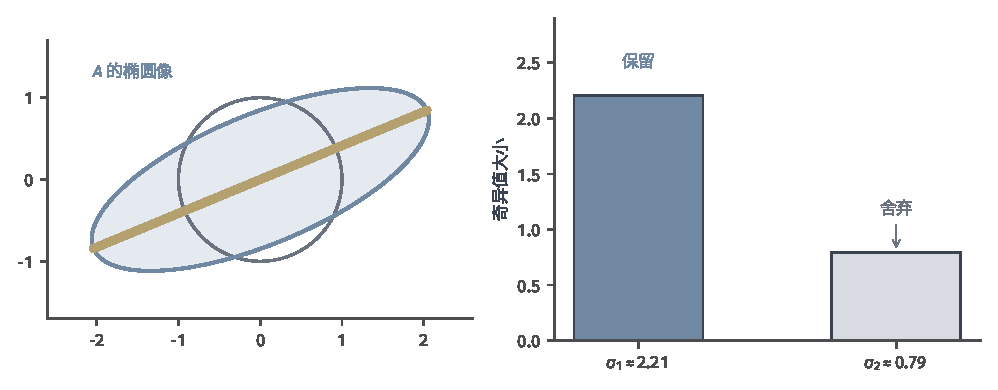
\includegraphics[width=168.998mm]{figures/00-shared/mathematical-preliminaries-upper/02-linear-spaces/matplotlib/ls-low-rank-truncation/ls-low-rank-truncation.pdf}
  \caption{低秩截断的几何。$\bm A=\left[\begin{smallmatrix}2&0.5\\0.5&1\end{smallmatrix}\right]$，
  灰圆为单位圆，蓝椭圆为$\bm A$的像。左：黄粗线段为秩一近似$\bm A_1=\sigma_1\bm v_1\bm v_1^\top$
  的像，椭圆被压成长$2\sigma_1$的线段；右：$\sigma_1\approx2.21$（保留）、$\sigma_2\approx0.79$
  （舍弃），算子范数误差$\lVert\bm A-\bm A_1\rVert_2=\sigma_2$。$\sigma_{1,2}=(3\pm\sqrt2)/2$。
  固定复算。}
  \label{fig:ls-low-rank-truncation}
\end{figure*}

\subsubsection{算法分析}

\paragraph{表示与计算代价}
截断SVD的好处在于表示代价。直接存储$\bm A$需要$md$个数；保存因子$\bm U_k$、$\sigma_1,\ldots,\sigma_k$与$\bm V_k$只需
\[
 k(m+d+1)
\]
个数。用$\bm A_k$乘向量时按
\[
 \bm A_k\bm x=\bm U_k\bigl(\bm\Sigma_k(\bm V_k^\top\bm x)\bigr)
\]
的顺序计算，依次需要约$dk$、$k$、$mk$次乘法，共$O(k(m+d))$次运算，而直接用$\bm A$乘向量需要$O(md)$次。

例如$m=d=1000$、$k=10$时，存储由$10^6$个数降为$20010$个数。形成完整的$\bm A_k=\bm U_k\bm W$约需$mdk$次乘法，只在需要矩阵本身或核验残差时才做。

这些是表示与后续作用的代价，不包括计算SVD本身的代价；后者取决于所用的数值算法，本书不作分析。

\paragraph{用途的区别}
第~\ref{chap:solution-error-regularization}章的截断SVD求解也用到$\bm A_k$，但那里是用它的伪逆稳定地求解方程；这里$\bm A_k$本身就是要评价的近似对象，评价标准是重建误差。$\bm A_k$的误差有多大、它在全部秩不超过$k$的矩阵中是否最好，由下一小节回答。

\subsection{最佳误差与最优性}
\label{sec:ls-truncated-svd-optimality}

\paragraph{截断SVD的误差}
截断SVD舍弃了后$r-k$项，误差应当由舍弃的奇异值决定。先把它算出来。设$0\leq k<r$，余下的部分是
\[
 \bm A-\bm A_k=\sum_{i=k+1}^r\sigma_i\bm u_i\bm v_i^\top .
\]
它仍由两组标准正交向量和降序的正系数$\sigma_{k+1}\geq\cdots\geq\sigma_r$组成，可以照第~\ref{sec:ls-svd-matrix-size}节的方法读出它的大小。

先看谱范数。把输入写成$\bm x=\sum_{i=1}^dc_i\bm v_i$，则
\[
 (\bm A-\bm A_k)\bm x=\sum_{i=k+1}^r\sigma_ic_i\bm u_i .
\]
由$\bm u_i$标准正交，
\[
 \lVert(\bm A-\bm A_k)\bm x\rVert_2^2=\sum_{i=k+1}^r\sigma_i^2c_i^2\leq\sigma_{k+1}^2\lVert\bm x\rVert_2^2,
\]
等号在$\bm x=\bm v_{k+1}$时成立。

再看Frobenius范数。由$\bm u_i^\top\bm u_j=\delta_{i,j}$，
\[
 (\bm A-\bm A_k)^\top(\bm A-\bm A_k)=\sum_{i=k+1}^r\sigma_i^2\bm v_i\bm v_i^\top ,
\]
取迹得Frobenius范数平方$\sum_{i>k}\sigma_i^2$。于是
\begin{equation}
\begin{gathered}
\lVert\bm A-\bm A_k\rVert_2=\sigma_{k+1}\\
\lVert\bm A-\bm A_k\rVert_{\mathrm F}
 =\Bigl(\sum_{i=k+1}^r\sigma_i^2\Bigr)^{1/2}.
\end{gathered}
\label{eq:ls-truncated-errors}
\end{equation}
Frobenius平方误差也可以由引理~\ref{lem:ls-low-rank-projection-error}读出：
\[
 \lVert\bm A\rVert_{\mathrm F}^2-\operatorname{tr}(\bm U_k^\top\bm A\bm A^\top\bm U_k)=\sum_{i\leq r}\sigma_i^2-\sum_{i\leq k}\sigma_i^2 .
\]
示例~\ref{ex:matrix-approximation-truncated-three-by-three}中$k=1$时，式~\eqref{eq:ls-truncated-errors}给出$\sqrt{1^2+1^2}=\sqrt2$与$\sigma_2=1$，与直接计算的$\bm E_1$一致。

\begin{example}[对角矩阵的截断误差]
\label{ex:ls-truncated-svd-diagonal}
取示例~\ref{ex:ls-low-rank-three-columns}中的$\bm A=\operatorname{diag}(3,2,1)$，奇异值为$3,2,1$，可取$\bm u_i=\bm v_i=\bm e_i$。截断得
\[
 \bm A_1=\operatorname{diag}(3,0,0),\qquad\bm A_2=\operatorname{diag}(3,2,0),
\]
残差为
\[
 \bm A-\bm A_1=\operatorname{diag}(0,2,1),\qquad\bm A-\bm A_2=\operatorname{diag}(0,0,1).
\]
$k=1$时平方误差$2^2+1^2=5$，谱范数误差$2$；$k=2$时平方误差与谱范数误差都是$1$。两者都与式~\eqref{eq:ls-truncated-errors}一致：
\[
 5=\sigma_2^2+\sigma_3^2,\qquad 2=\sigma_2,\qquad 1=\sigma_3 .
\]

平方误差$5$是只保留坐标直线$\bm e_1$时的损失，平方误差$1$是最佳坐标平面$\operatorname{span}\{\bm e_1,\bm e_2\}$的损失。
\end{example}

\paragraph{为什么还要比较全部候选}
两种误差记录的内容不同：Frobenius平方误差汇总所有舍弃方向，谱范数误差只记录最坏的单位输入方向。式~\eqref{eq:ls-truncated-errors}只是这一构造的误差，尚需证明其他秩不超过$k$的矩阵不能更小。

Frobenius范数的结论由上一小节的化归和迹极值得到。谱范数不能这样处理，因为
\[
 \lVert\bm M\rVert_2\leq\lVert\bm M\rVert_{\mathrm F},
\]
Frobenius误差的下界推不出谱范数误差的下界，需要另作证明。

谱范数下界的想法是：秩不超过$k$的$\bm X$至少把一个$(d-k)$维子空间送到零，这个子空间一定与前$k+1$个右奇异方向相交；在交点处，$\bm A-\bm X$的作用就是$\bm A$本身的作用，而$\bm A$在前$k+1$个方向上至少放大$\sigma_{k+1}$倍。

下面用一个例子说明这一想法。取$\bm A=\operatorname{diag}(3,2,1)$、$k=1$，并取一个不同于截断SVD的秩一候选：
\[
 \bm X=\begin{bmatrix}3&2&0\\0&0&0\\0&0&0\end{bmatrix}.
\]
它的核是$\{\bm x:3x_1+2x_2=0\}$，与$\operatorname{span}\{\bm e_1,\bm e_2\}$交于
\[
 \bm x=\frac1{\sqrt{13}}\begin{bmatrix}2\\-3\\0\end{bmatrix}.
\]
在这个单位向量上$\bm X\bm x=\bm0$，于是
\[
 (\bm A-\bm X)\bm x=\bm A\bm x=\frac1{\sqrt{13}}\begin{bmatrix}6\\-6\\0\end{bmatrix},
\]
它的长度为
\[
 \lVert\bm A\bm x\rVert_2=\sqrt{72/13}\approx2.353\geq\sigma_2=2 .
\]
所以这个候选的谱范数误差至少为$2.353$，不比截断SVD好。下面的定理对任意候选作同样的论证。

\begin{theorem}[Eckart--Young--Mirsky最佳低秩逼近]
\label{thm:ls-best-low-rank}
\label{thm:matrix-analysis-best-low-rank}
设$\bm A\in\mathbb R^{m\times d}$的秩为$r$，奇异值为$\sigma_1\geq\cdots\geq\sigma_r>0$。对$0\leq k<r$，
\begin{align}
 \min_{\operatorname{rank}\bm X\leq k}\lVert\bm A-\bm X\rVert_2
 &=\sigma_{k+1},
 \label{eq:matrix-analysis-best-rank-k-spectral}\\
 \min_{\operatorname{rank}\bm X\leq k}\lVert\bm A-\bm X\rVert_{\mathrm F}
 &=\Bigl(\sum_{i=k+1}^r\sigma_i^2\Bigr)^{1/2},
 \label{eq:matrix-analysis-best-rank-k-frobenius}
\end{align}
两个最小值都由截断SVD$\bm A_k$达到。
\end{theorem}
\begin{proof}
由式~\eqref{eq:ls-truncated-errors}，$\bm A_k$的两种误差恰为右端，只需证明任意秩不超过$k$的$\bm X$误差都不更小。$k=0$时只有$\bm X=\bm0$，结论即式~\eqref{eq:ls-truncated-errors}，下设$k\geq1$。

Frobenius情形。按第~\ref{sec:ls-low-rank-projection-error}节的做法，把$\bm X$的列空间补成一个$k$维子空间，取其标准正交基组成$\bm Y$，则$\bm X=\bm Y\bm C$。由引理~\ref{lem:ls-low-rank-projection-error}、定理~\ref{thm:matrix-analysis-trace-minimum}与式~\eqref{eq:matrix-analysis-frobenius-norm}，
\[
 \begin{aligned}
 \lVert\bm A-\bm X\rVert_{\mathrm F}^2
 &\geq\lVert\bm A\rVert_{\mathrm F}^2-\operatorname{tr}(\bm Y^\top\bm A\bm A^\top\bm Y)\\
 &\geq\sum_{i=1}^r\sigma_i^2-\sum_{i=1}^k\sigma_i^2=\sum_{i=k+1}^r\sigma_i^2 .
 \end{aligned}
\]

谱范数情形。由秩零度定理~\ref{thm:ls-rank-nullity}，
\[
 \dim\ker\bm X=d-\operatorname{rank}\bm X\geq d-k .
\]
子空间$\operatorname{span}\{\bm v_1,\ldots,\bm v_{k+1}\}$的维数为$k+1$（$k+1\leq r\leq d$）。两者维数之和超过$d$，由维数公式，它们有非零公共向量；取其中的单位向量$\bm x=\sum_{i=1}^{k+1}c_i\bm v_i$，$\sum_ic_i^2=1$。由$\bm X\bm x=\bm0$，
\begin{equation}
 \lVert(\bm A-\bm X)\bm x\rVert_2
 =\lVert\bm A\bm x\rVert_2
 =\Bigl(\sum_{i=1}^{k+1}\sigma_i^2c_i^2\Bigr)^{1/2}
 \geq\sigma_{k+1},
 \label{eq:ls-spectral-lower-bound}
\end{equation}
所以$\lVert\bm A-\bm X\rVert_2\geq\sigma_{k+1}$。
\end{proof}

在上面的秩一候选中，$c_1=2/\sqrt{13}$、$c_2=-3/\sqrt{13}$，式~\eqref{eq:ls-spectral-lower-bound}的中间量为
\[
 \sigma_1^2c_1^2+\sigma_2^2c_2^2=9\cdot\frac4{13}+4\cdot\frac9{13}=\frac{72}{13}\geq\sigma_2^2=4 ,
\]
与直接计算一致。

这一结论最早由Eckart与Young给出\scite{eckart1936}。定理覆盖任意秩不超过$k$的矩阵，而不只覆盖事先选定的投影形式：Frobenius情形借助第~\ref{sec:ls-low-rank-projection-error}节的化归把任意候选归入某个子空间，谱范数情形则直接利用候选矩阵的核。两种范数下的最小误差都由舍弃的奇异值决定：谱范数看最大的舍弃值$\sigma_{k+1}$，Frobenius范数看全部舍弃值的平方和。

\subsection{最优解的唯一性}
\label{sec:matrix-approximation-low-rank-uniqueness}

\paragraph{Frobenius情形}
最小误差唯一，达到最小误差的矩阵却未必唯一。示例~\ref{ex:matrix-approximation-truncated-three-by-three}中的$\bm A_2$与$\bm A_2'$已经说明了这一点。问题是：什么条件下最优矩阵只有一个？在有效的秩预算$1\leq k<r$下，Frobenius情形的答案由迹极值的取等条件决定，关键是截断位置两侧的奇异值是否有间隙。

\begin{theorem}[Frobenius最佳逼近的唯一性]
\label{thm:ls-best-low-rank-uniqueness}
设$1\leq k<r$且$\sigma_k>\sigma_{k+1}$，则$\bm A_k$是$\min_{\operatorname{rank}\bm X\leq k}\lVert\bm A-\bm X\rVert_{\mathrm F}$的唯一最优解。
\end{theorem}
\begin{proof}
设$\bm X$达到最小值，按定理~\ref{thm:ls-best-low-rank}的证明取$\bm Y$，写$\bm X=\bm Y\bm C$。证明中的两个不等号都须取等。第一个取等，由式~\eqref{eq:ls-low-rank-projection-split}得$\bm C=\bm Y^\top\bm A$，即
\[
 \bm X=\bm Y\bm Y^\top\bm A .
\]

第二个取等，即
\[
 \operatorname{tr}(\bm Y^\top\bm A\bm A^\top\bm Y)=\sum_{i=1}^k\sigma_i^2 .
\]
$\bm A\bm A^\top$的第$k$与第$k+1$个特征值为$\sigma_k^2>\sigma_{k+1}^2$，由定理~\ref{thm:matrix-analysis-trace-minimum}的取等条件，$\operatorname{range}(\bm Y)=\operatorname{span}\{\bm u_1,\ldots,\bm u_k\}$。

到同一子空间的正交投影是同一个矩阵，故$\bm Y\bm Y^\top=\bm U_k\bm U_k^\top$，从而
\[
 \bm X=\bm U_k\bm U_k^\top\bm A=\bm A_k .
\]
\end{proof}

$k=1$时，条件$\sigma_1>\sigma_2$正是第~\ref{sec:matrix-approximation-rank-one-solution}节秩一最优解唯一的条件。

间隙条件也确定了$\bm A_k$本身：$\sigma_k>\sigma_{k+1}$时，$\operatorname{span}\{\bm u_1,\ldots,\bm u_k\}$是$\bm A\bm A^\top$前$k$个特征值对应的特征空间之和，不随SVD的选取改变，$\bm A_k=\bm U_k\bm U_k^\top\bm A$也就与所选的奇异向量无关。示例~\ref{ex:matrix-approximation-truncated-three-by-three}中$k=1$时$\sigma_1=5>\sigma_2=1$，$\bm A_1$唯一；$k=2$时$\sigma_2=\sigma_3$，定理不适用。

截断跨过相等的正奇异值时，唯一性失败。例如$\bm A=\operatorname{diag}(2,1,1)$、$k=2$，下面两个矩阵都是最优解：
\[
 \operatorname{diag}(2,1,0),\qquad\operatorname{diag}(2,0,1).
\]
它们的残差分别是$\operatorname{diag}(0,0,1)$与$\operatorname{diag}(0,1,0)$，平方误差都是$1=\sigma_3^2$。这时“前$k$个奇异向量”本身就有不同选法，每种选法给出一个最优矩阵；三阶例中的$\bm A_2$与$\bm A_2'$也是这种情形。

\paragraph{谱范数情形}
谱范数下的最优矩阵即使有间隙也不唯一，所以间隙条件不能直接当成谱范数的唯一性保证。先说明对角矩阵的谱范数。$\bm D=\operatorname{diag}(a_1,\ldots,a_m)$满足
\[
 \lVert\bm D\bm x\rVert_2^2=\sum_ia_i^2x_i^2\leq\max_ia_i^2\,\lVert\bm x\rVert_2^2 ,
\]
在绝对值最大的对角元所在的坐标向量处取等，故
\[
 \lVert\bm D\rVert_2=\max_i\lvert a_i\rvert .
\]
取$\bm A=\operatorname{diag}(3,2,1)$、$k=1$，候选$\bm X=\operatorname{diag}(t,0,0)$给出残差$\operatorname{diag}(3-t,2,1)$，于是
\[
 \lVert\bm A-\bm X\rVert_2=\max(\lvert3-t\rvert,2).
\]
$1\leq t\leq5$时它都等于最小值$2$，尽管$\sigma_1=3>\sigma_2=2$。例如$t=2$时残差是$\operatorname{diag}(1,2,1)$，最坏方向仍是$\bm e_2$。谱范数只看最坏方向，最坏方向之外的偏差在一定范围内可以随意改变。

Frobenius范数则不同：同一族候选的平方误差是
\[
 \lVert\bm A-\bm X\rVert_{\mathrm F}^2=(3-t)^2+5 ,
\]
只在$t=3$时取到最小值$5$。

\paragraph{边界情形与适用范围}
边界情形$k=0$与$k\geq r$已在第~\ref{sec:matrix-approximation-problem}节回答，最优矩阵分别是$\bm0$与$\bm A$本身，不需要套用间隙判据。

本节的最优性依赖两个前提：允许集合是全部秩不超过$k$的矩阵，误差是谱范数或Frobenius范数。额外要求近似矩阵非负或因子稀疏时，允许集合缩小，$\bm A_k$可能不再可行。改用逐元素加权的平方误差
\[
 \sum_{i,j}w_{i,j}(a_{i,j}-x_{i,j})^2
\]
时，误差一般不再按正交投影分解，引理~\ref{lem:ls-low-rank-projection-error}失效。这些情形下截断SVD一般不再是最优解，最优性需要重新论证；下一节处理其中能够化归的一类加权误差。
